\section{Contexte et définition du problème}


	\subsection{Danger des batteries Li-Ion}
	% merger avec la version à l'école
	
		\subsection{Système de protection et de gestion de batterie}
		
		% TODO: Petite description d'un BMS
		
		Il est important de comprendre les différentes composantes formant le système de protection et de gestion de batterie.
		
			\paragraph{}
			\textbf{Cellule:} C'est la plus petite unité composant un système. Les cellules sont des accumulateurs chimiques pouvant avoir avoir une formes cylindriques, prismatiques ou en sachet.  
			
			\paragraph{}
			\textbf{Module:} Les cellules sont regrouper en parralèles pour former des modules. De cette façon, on peut additionner le courant vennant des cellules. Les modules peuvent être remplacer dans un système.
			
			\paragraph{}
			\textbf{Batterie:} On dispose les modules en série pour former la batterie. On augmente ainsi la tension pour l'application voulue.
			
			\paragraph{}
			\textbf{Système de protection:} Cette composante effectue des mesures sur les modules. On mesure entre autre la tension, le courant et la température. Cela permet de savoir si les cellules opèrent à l'intérieur des caractéristiques fourni par le manufacturier des cellules. Il s'assure également que les modules soient balancé pour éviter une surtension des modules lors de la recharge. Il commande aussi les périphériques auxilières, tels que les ventilateurs de refroidissement.
			
			
			\paragraph{}
			\textbf{Système de gestion:} Il est nécessaire de faire une bonne gestion pour s'assurer du bon fonctionnement de la batterie. Le système de gestion calcul donc l'état de charge, l'état de santé et les limites de puissances. Le système communique ces informations à d'autres systèmes avec un protocole de communication. Il gère également les contacteurs connectant la batterie avec la charge et la recharge.
		
	
	\subsection{Projet spécial}
	% merger avec la version à l'école
	Dans le cadre du cours ELE791, une équipe de trois étudiant en génie électrique de l'École de technologie supérieur feront la conception d'un système de protection et de gestion de batterie. Ce cours permet aux étudiants de réaliser un projet d'initiation à la recherche ou un projet destiné à un club étudiant participant aux diverse compétitions d'ingénierie. Un rapport technique et une présentation orale doivent être effectués au terme de ce projet. Or, l'équipe fait partie du club étudiant Éclipse et réalisera le système de protection et de gestion de batterie du dixième prototype de ce club.
	
		
	\subsection{Club étudiant Éclipse}
	
		\paragraph{}
		Éclipse est un club étudiant composé d'une quarantaine d'étudiants en ingénierie qui ont pour objectif de construire une véhicule alimenter par l'énergie solaire à l'aide de panneaux photovoltaïques. Depuis sa fondation en 1992, neuf prototypes ont été construit en y intégrant les technologies de pointes disponibles au moment de leurs conceptions. Similaire aux voitures électriques, le véhicule solaire possède une chaîne de traction électrique comme moyen de propulsion. Les moteurs roues  CSIRO sont alimentés par des entraînement électrique qui sont à leur tour alimentés bar une batterie. Depuis quelques années, l'équipe s'est tourné vers l'utilisation d'accumulateurs au Li-ion. Il est donc nécessaire d'avoir un système de protection et de gestion de batterie.
		
		\paragraph{}
		Une des philosophies du club est de concevoir par les étudiants le plus de modules possible. Le temps de développement du dernier système de protection et de gestion de batterie à pris environ 7 ans et comme la conception d'un nouveau véhicule se fait à tous les deux ans, la disposition des batteries changent beaucoup. C'est pourquoi les deux derniers prototypes ont utilisés des systèmes acheter par manque de temps. L'intégration de système provenant de compagnie accélère le temps de fabrications du véhicule mais ne permet pas le contrôle total du système et l'expertise de conception de ces systèmes se perd au sein du club puisqu'il y a un gros roulement des étudiants. Il faut également des systèmes fiables et robustes, ce qui peut être difficile à concevoir lorsque ce système est aussi critique qu'un système de protection et de gestion de batterie. Une défaillance de ce système pourrait mener la destruction partiel ou total du véhicule et la vie du pilote est en jeu. D'autant plus que le véhicule solaire sera soumis à plusieurs épreuves dans des conditions de route réelles et en circuit fermé durant les compétitions.
		
	
	\subsection{Compétitions}
	
	
	\subsubsection{ASC2016}
	
	Scruteneering
	
	\subsubsection{Compétitions futures}
	
	Règlements
	
	
	FSGP2017
	ASC2018
	WSC2019
	
	
	
	\subsection{Rétrocompatibilité}
	
	
	
	BMS Lithium Balance
	
	%\begin{figure}[h!]
	%	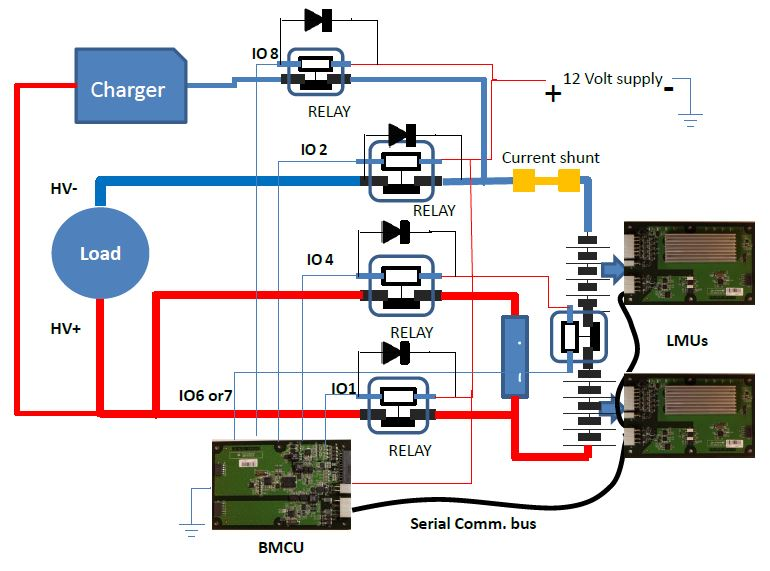
\includegraphics[width=\linewidth]{Hardware.jpg}
	%	\caption{Disposition matériel du système de protection}
	%	\label{fig:Disposition matériel}
	%\end{figure}
	%
	%Pin out
	%
	%\begin{figure}[h!]
	%	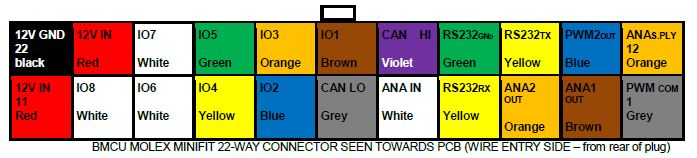
\includegraphics[width=\linewidth]{Pinout.jpg}
	%	\caption{Brochage du connecteur}
	%	\label{fig:Brochage1}
	%\end{figure}
	%
	%\begin{figure}[h!]
	%	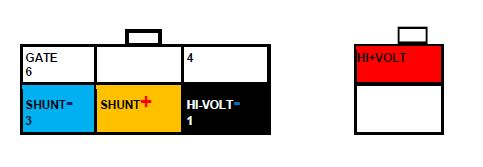
\includegraphics[width=\linewidth]{Pinout2.jpg}
	%	\caption{Brochage du connecteur}
	%	\label{fig:Brochage2}
	%\end{figure}
	%

